\documentclass[a4paper,landscape,8pt,fleqn]{scrartcl}
\usepackage[english]{babel}
\usepackage[utf8]{inputenc}
\usepackage[a4paper, landscape, margin=1.1cm]{geometry}
\usepackage{latexsym}
\usepackage{multicol}
\usepackage{amsmath}
\usepackage{amsfonts}
\usepackage{amssymb}
\usepackage{array}
\usepackage{graphicx}
\usepackage{booktabs}
\usepackage{empheq}			% emphasize (box) equations
\usepackage{float}				% add H as an option for floats
\usepackage{parskip}			% add no indentation to new paragraphs
\usepackage{enumitem}		% description lists
\usepackage{fancyhdr}
\usepackage{lastpage}
\usepackage{framed}
\usepackage{bm}					% bold math symbols

\newcommand{\SummaryTitle}{Asset Management: Advanced Investments}
\newcommand{\SummaryAuthor}{Fabian MARBACH}
\newcommand{\SummarySemester}{Spring Semester 2016}

\pagestyle{plain}
\columnsep 30pt
\columnseprule .4pt

\setlength{\mathindent}{0.1cm}

\newcommand*\widefbox[1]{\fbox{\hspace{2em}#1\hspace{2em}}}		% required for boxing several lines of equations at once

\renewcommand*{\familydefault}{\sfdefault}		% set font to default sans-serif

\renewcommand{\labelitemi}{\tiny$\blacksquare$}		% change symbol of itemized lists
\setlist[itemize]{leftmargin=0.4cm}								% reduce indentation of itemized lists
\renewcommand{\labelenumi}{(\roman{enumi})}			% change counter of enumerated lists
\setlist[enumerate]{leftmargin=0.4cm}							% reduce indentation of enumerated lists

\renewcommand{\arraystretch}{1}
\renewcommand{\emph}[1]{\textbf{#1}}

%\allowdisplaybreaks	% equations can be split on two pages/columns

\graphicspath{{images/}}

\pagestyle{fancy}
\fancyhead{}
\setlength{\headheight}{0pt}
\setlength{\footheight}{14pt}
\renewcommand{\headrulewidth}{0pt}
\renewcommand{\footrulewidth}{0.5pt}
\lfoot{\SummaryAuthor}
\cfoot{p \thepage\ / \pageref{LastPage}}
\rfoot{\SummaryTitle}

\usepackage{parskip}	% add no indentation to new paragraphs

\makeatletter
\renewcommand{\section}{\@startsection{section}{1}{0mm}%
{-2\baselineskip}{0.8\baselineskip}%
{\hrule depth 0.2pt width\columnwidth\hrule depth1.5pt
width0.25\columnwidth\vspace*{1.2em}\Large\bfseries}}
\makeatother

\makeatletter
\renewcommand{\subsection}{\@startsection{subsection}{1}{0mm}%
{-2\baselineskip}{0.8\baselineskip}%
{\hrule depth 0.2pt width\columnwidth\hrule depth0.75pt
width0.25\columnwidth\vspace*{1.2em}\large\bfseries}}
\makeatother

\makeatletter
\renewcommand{\subsubsection}{\@startsection{subsubsection}{1}{0mm}%
{-2\baselineskip}{0.8\baselineskip}%
{\hrule depth 0.2pt width\columnwidth\vspace*{1.2em}\normalsize\bfseries}}
\makeatother

\newcommand{\Mx}[1]{\begin{bmatrix}#1\end{bmatrix}}
\newcommand{\dd}[2]{\frac{\text{d}#1}{\text{d}#2}}
\newcommand{\DD}[2]{\frac{\text{D}#1}{\text{D}#2}}
\newcommand{\deidei}[2]{\frac{\partial#1}{\partial#2}}
\newcommand{\Lbrace}[1]{\left\{\begin{array}{ll}#1\end{array}\right.} % left brace with text

% Declare mathematical operators
\DeclareMathOperator{\erf}{erf}					% error function
\DeclareMathOperator{\Var}{Var}				% variance
\DeclareMathOperator{\Varn}{Varn}			% variation
\DeclareMathOperator{\QV}{QV}				% quadratic variation
\DeclareMathOperator{\Cov}{Cov}				% covariance
\DeclareMathOperator{\Ber}{Ber}				% Bernoulli distribution
\DeclareMathOperator{\Bin}{Bin}				% Binomial distribution
\DeclareMathOperator{\Geom}{Geom}		% Geometric distribution
\DeclareMathOperator{\Poi}{Poi}					% Poisson distribution
\DeclareMathOperator{\Gammaa}{Gamma}	% Gamma distribution
\DeclareMathOperator{\Cau}{Cau}				% Cauchy distribution
\DeclareMathOperator{\Adj}{Adj}				% Adjoint
\DeclareMathOperator{\Bias}{Bias}				% Bias of an estimator
\DeclareMathOperator{\rank}{rank}				% rank of a matrix
\DeclareMathOperator{\diag}{diag}				% diagonal matrix
\DeclareMathOperator{\VaR}{VaR}				% Value-at-Risk
\DeclareMathOperator{\ES}{ES}					% Expected shortfall
\DeclareMathOperator{\R}{R}						% Risk measure
\DeclareMathOperator{\RC}{RC}					% Risk contribution
\DeclareMathOperator{\D}{D}						% Diversification index
\DeclareMathOperator{\DR}{DR}					% Diversification ratio
\DeclareMathOperator{\tr}{tr}						% trace
\DeclareMathOperator{\IW}{IW}					% inverted Wishart distribution
\DeclareMathOperator{\SR}{SR}					% Sharpe ratio

\begin{document}
\part*{Summary: \SummaryTitle}
\SummaryAuthor, \SummarySemester
\begin{multicols*}{3}
%\tableofcontents
%\end{multicols}
%{\vspace*{0.3cm}}
%{\hrule depth 0.2pt}
%{\vspace*{0.3cm}}
%\begin{multicols}{2}
\raggedcolumns
\newpage

\section*{Useful expressions}

\paragraph{Mean, variance and covariances of portfolios}
\begin{itemize}
\item return of portfolio: $R_{\bm w} = \bm w^\top \bm \mu$
\item variance of a portfolio:
\begin{align*}
\sigma^2(\bm w) &= \bm w^\top \Sigma \bm w = \sum_{i=1}^n w_i^2 \sigma_i^2 + 2 \sum_{i > j} w_i w_j \rho_{ij} \sigma_i \sigma_j
\end{align*}
\item covariance of two portfolios $\bm w_p, \bm w_q$: $\Cov[R_p, R_q] = \bm w_p^\top \Sigma \bm w_q$
\item covariance of a single asset $i$ with a portfolio $\bm w$: \\
$\Cov[R_i, R_{\bm w}] = (\Sigma \bm w)_i$
\end{itemize}

\paragraph{Sharpe ratio of a portfolio}
\begin{align*}
\SR(\bm w) &= \frac{\mu(\bm w) - R_f}{\sigma(\bm w)}
\end{align*}

\paragraph{Linear Algebra}
\begin{itemize}
\item product rule: $(A B)^\top = B^\top A^\top$ \\
and: $(A_1 A_2 \cdots A_k)^\top = A_k^\top \cdots A_2^\top A_1^\top$
\item transpose of an inverse: $(A^{-1})^\top = (A^\top)^{-1}$
\item dot-product of two vectors: $a^\top b = b^\top a \in \mathbb{R}$
\end{itemize}

\section{Mean-variance paradigm}

\paragraph{Main advantage of the MV paradigm}
\begin{itemize}
\item The MV paradigm provides a simple framework to construct and select portfolios, based on \textit{expected performance} of investments and \textit{risk appetite} of investors.
\end{itemize}

\paragraph{MV critique and approaches to overcome MV shortcomings}
\begin{itemize}
\item The MV approach relies on \textit{variance as a risk measure}.
\begin{itemize}
\item An investor might not think in terms of utility functions but first wants to make sure that a certain amount of the principal is reserved.
\end{itemize}
$\leadsto$ portfolio optimization based on other risk measures, e.g. based on \textit{VaR} or \textit{ES}
\item There is a \textit{high rebalancing activity} / high \textit{instability of optimal portfolio weights $\bm w$} / \textit{high sensitivity to input parameters} (i.e. return estimates).
\begin{itemize}
\item Even small and selected changes in expected returns lead to huge unrealistic shifts/fluctuations in asset weights.
\item Furthermore, MV portfolios often seem counterintuitive and inexplicable.
\end{itemize}
This is caused by: \textit{Error maximization} / high \textit{estimation risk:}
\begin{itemize}
\item Most of the estimation risk is due to errors in estimates of expected returns (not estimates of risk).
\item MV optimization exacerbates effect of sampling errors since it takes advantage of unusually high means and low variances.
\item Estimation risk arises naturally, as samples are not sufficiently large and market structures change over time.
\end{itemize}
$\leadsto$ \textit{resampling methods}, \textit{constrained optimization} (e.g. sets constraints on weights), \textit{robust optimization} (considers uncertainty in unknown parameters directly and explicitly), \textit{shrinkage estimators}, \textit{Black-Litterman model}, \textit{Risk-Budgeting} (does not employ explicit forecasts of asset returns)
\item There is a \textit{bias in estimated performance}.
\begin{itemize}
\item The MV approach promises far more than it delivers.
\item The actual frontier always lies below the estimated frontier.
\end{itemize}
$\leadsto$ \textit{robust optimization}
\item MV optimization may result in \textit{under-diversified} strategies.
\begin{itemize}
\item E.g. during the financial crisis, risk contribution of equities far exceeded their forecast limits --- partly due to a realised jump in realised equity correlation.
\end{itemize}
$\leadsto$ \textit{Risk budgeting} (risk factors exhibit by far lower correlation than equity)
\item MV is only data-driven, i.e. \textit{subjective views} are not considered. \\
$\leadsto$ the \textit{Black-Litterman approach} incorporates both market data and subjective views.
\item There is \textit{no quantification of confidence} in estimated portfolio returns $\mu_p$. \\
$\leadsto$ \textit{robust optimization}, \textit{Black-Litterman}, \textit{Bayesian approaches}
\item MV is only a \textit{one-periodical} approach. \\
$\leadsto$ \textit{multi-period approaches} (discrete or continuous time)
\end{itemize}

\subsection{MV without Riskless Asset}

\paragraph{Definition}
\begin{itemize}
\item Given: $n$ risky assets w/ mean vector $\bm \mu \in \mathbb{R}^n$ and covariance matrix $\Sigma \in \mathbb{R}^{n \times n}$
\item Chose: target mean return $\mu_p$
\item Then: $P$ is the corresponding minimum-variance portfolio (MVP) iff:
\begin{itemize}
\item $P$ has minimal portfolio variance: $\bm w_p^\top \Sigma \bm w_p = \min_{\bm w} \bm w^\top \Sigma \bm w$
\item $P$ has target return $\mu_p$: $\bm w_p^\top \bm \mu = \mu_p$
\item $w$ is a weight vector: $\bm w_p^\top \bm  1 = 1$
\end{itemize}
\end{itemize}

\paragraph{Optimal weigths}
\begin{itemize}
\item without any restrictions on the portfolio weights, the weights of the MVF for given $\mu_p$ are:
\begin{align*}
\bm w_p &= \Sigma^{-1} (\mu_p \bm k_1 + \bm k_2), \quad \bm k_1 = \frac{c \bm \mu - b \bm 1}{d}, \quad \bm k_2 = \frac{a \bm 1 - b \bm \mu}{d}
\end{align*}
with:
\begin{align*}
a &= \bm \mu^\top \Sigma^{-1} \bm \mu, & b &= \bm \mu^\top \Sigma^{-1} \bm 1 \\
c &= \bm 1^\top \Sigma^{-1} \bm 1, & d &= ac - b^2
\end{align*}
\end{itemize}

\paragraph{Black's separation theorem}
\begin{itemize}
\item Any portfolio of MVPs is also an MVP.
\item The MVF can be generated by any two distinct MVPs.
\end{itemize}

\paragraph{Mean-Variance Frontier}
\begin{itemize}
\item \emph{mean-variance frontier (MVF):} set of all portfolios with mean return $\mu_p$ that solve above's minimization problem, i.e. with:
\begin{align*}
\mu_p &= \frac{b}{c} + \sqrt{\frac{d}{c} \left( \sigma_p^2 - \frac{1}{c} \right)}
\end{align*}
\item \emph{efficient frontier:} upper part of the MVF
\item \emph{inefficient frontier:} lower part of the MVF
\end{itemize}
Implications:
\begin{itemize}
\item Covariance of a MVP $\bm w_p$ with any asset or portfolio $\bm w_q$ (not necessarily on the MVF) is:
\begin{align*}
\Cov \left[ R_p, R_q \right] &= \frac{c}{d} \left( \mu_p - \frac{b}{c} \right) \left( \mu_q - \frac{b}{c} \right) + \frac{1}{c}
\end{align*}
which can also be written as:
\begin{align*}
\Cov \left[ R_p, R_q \right] &= e \left( \mu_p - f \right) \left( \mu_q - F \right) + g
\end{align*}
with:
\begin{align*}
e = \frac{c}{d}, \qquad f = \frac{b}{c}, \qquad g = \frac{1}{c}
\end{align*}
\item Covariance of two efficient MVPs is at least $\frac{1}{c} > 0$.
\item Covariance between two inefficient MVPs is always positive.
\end{itemize}

\paragraph{Global MVP (gMVP)}
\begin{itemize}
\item return: $\mu_g = \frac{b}{c}$, variance: $\sigma_g^2 = \frac{1}{c}$
\item optimal weights: $\bm w_g = \frac{1}{c} \Sigma^{-1} \bm 1$
\end{itemize}
Furthermore:
\begin{itemize}
\item covariance of any asset or portfolio return $R_p$ with the gMVP is:
\begin{align*}
\Cov \left[ R_g, R_p \right] = \frac{1}{c}
\end{align*}
\end{itemize}

\subsection{Zero Beta Portfolio}

\paragraph{Zero Beta Portfolio}
For each MVP $\bm w_p$, except for the gMVP, $\exists$ a unique MVP, the zero-beta MVP w.r.t. $\bm w_p$, that has zero covariance with $\bm w_p$. \\
\textit{Remarks:}
\begin{itemize}
\item In the absence of the risk-free rate, the efficient frontier consists of those MVPs with return $\mu_p$ equal or higher than the return of the gMVP $\mu_g$.
\item The return of the gMVP $\mu_g$ is equal or higher than the return of any zero-beta portfolio $\mu_{0p}$.
\item Thus it holds: $\mu_p \geq \mu_g \geq \mu_{0p}$
\end{itemize}

\paragraph{Beta Replication}
Every portfolio (not necessarily an MVP, $\mu_q$) has a beta representation in terms of a MVP ($\mu_p$) and a portfolio orthogonal to the MVP ($\mu_{0p}$):
\begin{align*}
\mu_q &= \mu_{0 p} + \beta_{pq} (\mu_p - \mu_{0p}), \qquad \beta_{pq} = \frac{\Cov \left[ R_p, R_q \right]}{\sigma_p^2}
\end{align*}
\textit{Remarks:}
\begin{itemize}
\item All zero-beta portfolios lie on a horizontal line.
\item Any feasible mean-variance combination can be constructed from any MVP $\bm w_p$ and some $\bm w_{0q}$, which is orthogonal to $\bm w_p$ (but not necessarily a MVP).
\end{itemize}

\paragraph{Existence of Zero Beta portfolios}
\begin{itemize}
\item Zero Beta portfolios only exist if \textit{short-sales} are allowed. \\
I.e. if there are short-sales constraints, then the Zero Beta portfolio does generally not exist.
\item There exists no Zero Beta portfolio for the \textit{GMV}.
\end{itemize}

\subsection{MV with Risk-Free Asset}

In presence of a risk-free asset:
\begin{itemize}
\item \textit{Given:} vector of excess returns of the assets over the risk-free rate, i.e. $\bm \mu^e = \bm \mu - \bm 1 R_f$, covariance matrix $\Sigma$
\item \textit{Choose:} target return $\mu_p$
\item \textit{Then:} the optimization problem reads:
\begin{align*}
\min_{\bm w_p} \bm w_p^\top \Sigma \bm w_p, \qquad \text{s.t. } \mu_p = R_f + (\bm \mu - \bm 1 R_f)^\top \bm w_p
\end{align*}
Note that the previous constraint $\bm 1^\top w = 1$ is not anymore necessary.
\item \textit{Result:} the weights $\bm w_p$ of the risky assets of the corresponding MVP and its variance are:
\begin{align*}
\bm w_p &= \frac{\mu_p - R_f}{(\bm \mu^e)^\top \Sigma^{-1} \bm \mu^e} \Sigma^{-1} \bm \mu^e \quad
\sigma_p = \frac{\mu_p - R_f}{(\bm \mu^e)^\top \Sigma^{-1} \bm \mu^e} \sqrt{(\bm \mu^e)^\top \Sigma^{-1} \bm \mu^e}
\end{align*}
and the fraction $1 - \bm 1^\top R_f$ is invested in the risk-free asset.
\end{itemize}

\paragraph{Tobin's Separation Theorem}
The relative portfolio fraction is independent of the choice of the targeted portfolio return $\mu_p$. \\
Implications:
\begin{itemize}
\item Every investor's portfolio decision is the same.
\item Only difference: relative portion between the risky protfolio and the risk-free rate $R_f$, which depends on the investor's risk-aversion.
\end{itemize}

\paragraph{Tangency portfolio}
The tangency portfolio $\bm w_T$ (with maximal Sharpe ratio) is characterized by:
\begin{align*}
\bm w_T &= \frac{\Sigma^{-1} \bm \mu^e}{\bm 1^\top \Sigma^{-1} \bm \mu^e} = \frac{\Sigma^{-1} (\bm \mu - \bm 1 R_f)}{b - c R_f} \\
\mu_T &= R_f + \frac{(\bm \mu^e)^\top \Sigma^{-1} \bm \mu^e}{\bm 1^\top \Sigma^{-1} \bm \mu^e}, \qquad
\sigma_T = \frac{\sqrt{(\bm \mu^e)^\top \Sigma^{-1} \bm \mu^e}}{\bm 1^\top \Sigma^{-1} \bm \mu^e}
\end{align*}
\textit{Remarks:}
\begin{itemize}
\item The tangency portfolio must consist of all assets available to investors, and each asset must be held in proportion to its relative market capitalization ($\equiv$ market portfolio)
\item Note that since $\bm w_T$ is independent of $\mu_p$, this proves Tobin's separation theorem.
\end{itemize}

%\subsection{MV with Liabilities}

\subsection{CAPM}

\paragraph{CAPM}
\begin{itemize}
\item The CAPM determines a theoretically appropriate required rate of return of an asset, if that asset is to be added to an already well-diversified portfolio, given that asset's non-diversifiable risk.
\item The CAPM takes the following aspects into account:
\begin{itemize}
\item asset's sensitivity to non-diversifiable risk (=systematic risk or market risk)
\item expected return of the market
\item expected return of a theoretical risk-free asset.
\end{itemize}
\end{itemize}

\paragraph{Assumptions of the CAPM}
\begin{itemize}
\item variance of returns is an adequate measurement of risk \\
(justified e.g. in case of a quadratic utility function)
\item investors are \textit{rational} and \textit{risk-averse}
\item investors are price-takers and can lend and borrow any amount under the same risk-free rate
\item all investors have access to the \textit{same information}
\item investors do not have \textit{preferences} between markets and assets, i.e. investors choose assets soley based on their risk-return profile
\item \textit{homogenous expectations assumption:} investors agree on the risk and expected return of all assets
\item \textit{no taxes}, \textit{no transaction costs}
\item assets are \textit{infinitely divisible}
\end{itemize}

\paragraph{Capital market line/security market line}
\begin{itemize}
\item All optimal portfolios $\bm w^\ast$ are on the \textit{capital market line:}
\begin{align*}
\mu^\ast &= R_f + \frac{\mu_m^e}{\sigma_m} \sigma^\ast
\end{align*}
with $\mu_m^e$ and $\sigma_m$ the parameters from the market portfolio.
\item This can also be written in terms of the \textit{security market line:}
\begin{align*}
\mu_i = R_f + \beta_i (\mu_M - R_f)
\end{align*}
where $R_f$ is the risk-free rate of return and $\mu_M$ is the return of the market portfolio. \\
Consequently, the term $\mu_M - R_f$ denotes the \textit{market excess return} or \textit{market risk premium}.
\end{itemize}

\paragraph{Beta representation}
For any portfolio or asset $i$, there is a beta representation, i.e.
\begin{align*}
\mu_i^e &= \beta_i \mu_m^e = \frac{\Cov[R_i,R_m]}{\Var[R_m]} \mu_m^e = \frac{\rho_{im} \sigma_i \sigma_m }{\sigma_m^2} \mu_m^e
\end{align*}
\textit{Remarks:}
\begin{itemize}
\item The graph $(\mu_i,\beta_i)$ is called the \emph{security market line}.
\item While \textit{standard deviation} measures risk arising from both systematic and unsystematic sources, the \textit{beta} only measures the risk w.r.t. to the variance from the market portfolio.
\item \emph{Low beta anomaly:} \\
Historically, low beta stocks have offered a combination of low risks and high returns.
\end{itemize}

\paragraph{CAPM applied to portfolios}
\begin{itemize}
\item If an investor wants to achieve a certain return $\mu_p$ by investing in the market portfolio and the risk-free asset, the corresponding beta $\beta_p$ can computed as:
\begin{align*}
\beta_p &= \frac{\mu_p - R_f}{\mu_M - R_f}
\end{align*}
\item The corresponding risk $\sigma_p$ can then be computed via:
\begin{align*}
\sigma_p = \beta_p \sigma_M
\end{align*}
\item Since the $\beta$ of a portfolio is simply the weighted sum of the assets' betas, the $\beta$ directly determines the ratio that has to be invested in the market portfolio, while the ratio $1-\beta$ determines the investment in the risk-free asset.
\item The relationship between the \emph{price of an asset $i$} and its expected return $\mu_i$ is given by:
\begin{align*}
P_i &= \frac{\mathbb{E}[X_i]}{1+\mu_i}
\end{align*}
where $\mathbb{E}[X_i]$ is the expected cash-flow of asset $i$.
\end{itemize}

\paragraph{Differences between the CAPM and the MV model}
While MV only looks at the optimization of a \textit{single investor}, the CAPM also considers the impact of this optimization on an aggregate market level by using equilibrium arguments.

\section{Downside Risk Measures}

\subsection{Motivation}

\paragraph{Semivariance}
In the MV approach, variance penalizes over- and underperformance equally. \\
Semivariance is concerned only with the adverse deviations and is defined as:
\begin{align*}
\sigma_{P,\min}^2 = \mathbb{E} \left[ \min \left( \sum_{i=1}^n w_i (R_i - \mu_i), 0 \right) \right]
\end{align*}
Generalization of semivariance: lower partial moment of risk measures.

\paragraph{Lower Partial Moments (LPMs)}
\begin{align*}
\sigma_{P,q,R_0} &= \mathbb{E} \left[ \max(R_0 - R_P,0)^q \right]^{1/q}
\end{align*}
with a \textit{power index} $q$ and \textit{target rate of return} $R_0$.
\begin{itemize}
\item Variance and semivariance are consistent with an investor having quadratic utility only. LPMs are consistent with a much wider class of vNM utility functions.
\item cases:
\begin{itemize}
\item $0 < q < 1$: risk-seeking investor
\item $q=1$: risk-neutral investor
\item $1 < q$: risk-averse investor
\item $q=2$: semivariance / semivolatility
\end{itemize}
\end{itemize}

\subsection{Value at Risk (VaR) and Expected Shortfall (ES)}

\subsubsection{Value at Risk (VaR)}

\paragraph{Value-at-Risk (VaR)}
\begin{itemize}
\item $\VaR_\alpha(X,n)$ is the \textit{maximum potential loss} that a portfolio $X$ can suffer in the 100$\alpha$\% \textit{best} cases in $n$ days.
\item $\VaR_\alpha(X,n)$ is the \textit{minimum potential loss} that a portfolio $X$ can suffer in the 100$(1-\alpha)$\% \textit{worst} cases in $n$ days.
\item Given a RV $X$ on $(\Omega, \mathcal{A}, \mathbb{P})$ and a scalar $\alpha \in (0,1)$,
\begin{align*}
\VaR_\alpha(X,n) \equiv -\sup \lbrace x : \mathbb{P}[X < x] \leq 1-\alpha \rbrace, \qquad \alpha \in [0,1)
\end{align*}
i.e. $\VaR_\alpha(X,n)$ defines a quantity such that
\begin{align*}
\mathbb{P}[X \geq -\VaR_\alpha(X,n)] \geq \alpha
\end{align*}
i.e. $\VaR_\alpha$ is a $\alpha$ quantile. Usually, $\alpha \in [0.5,1)$.
\item Note that $\VaR_\alpha = - \VaR_{1-\alpha}$.
\end{itemize}

\paragraph{VaR return}
\begin{itemize}
\item The $100\alpha$\%-VaR is the return $v$ s.t. $F(-v) = 1-\alpha$, $\alpha \in(0.5,1)$ and $F$ the CDF of the portfolio's return.
\item Mathematically:
\begin{align*}
v(r_w,\alpha) &= z_\alpha \sqrt{\bm w^\top \Sigma \bm w} - \bm w^\top \bm \mu = z_\alpha \sigma_{r_w} - \mu_{r_w}
\end{align*}
with $z_\alpha = \Phi^{-1}(\alpha)$, $\Phi$ the standard normal distribution, and $r_w$ the return of portfolio $\bm w$, $r_w \sim \mathcal{N}(\bm w^\top \bm \mu, \bm w^\top \Sigma \bm w)$.
\end{itemize}

\paragraph{$(\mu, \VaR)$-optimization}
\begin{itemize}
\item Optimization problem:
\begin{align*}
\min_{\bm w \in \mathcal{W}} z_\alpha \sigma_{r_w} - \mu_{r_w}, \qquad \text{s.t. } \mathbb{E}[r_w] = \bar r
\end{align*}
with $z_\alpha = \Phi^{-1}(\alpha) > \sqrt{\frac{d}{c}}$ a necessary and sufficient condition for this portfolio. \\
Since the return of a MVP is given by $\mu_p = \frac{b}{c} + \sqrt{\frac{d}{c} \left( \sigma_p^2 - \frac{1}{c} \right)}$ and the variance of the GMV portfolio is $\sigma_g = \frac{1}{\sqrt{c}}$, this can be rewritten as:
\begin{align*}
\min_{\sigma \in [\sigma_g, \infty)} \sigma z_\alpha - \left( \frac{b}{c} + \sqrt{\frac{d}{c} \left( \sigma_p^2 - \frac{1}{c} \right)} \right)
\end{align*}
\item The set of solutions build the \textit{mean-VaR boundary}, which is given as:
\begin{align*}
\left\lbrace (v(r,\alpha), \mu_r) \quad : \quad \frac{(v(r,\alpha) + \mu_r)^2}{z_\alpha^2 / c} - \frac{(\mu_r - b/c)^2}{d/c^2} = 1 \right\rbrace
\end{align*}
\item The minimum VaR portfolio existis iff $\alpha > \Phi(\sqrt{d/c})$. The weights are given as:
\begin{align*}
\bm w_m &= \Sigma^{-1} \left(  \left( \frac{b}{c} + \sqrt{\frac{d}{c} \left( \frac{z_\alpha^2}{c z_\alpha^2 - d} - \frac{1}{c} \right)} \right) \bm k_1 + \bm k_2 \right)
\end{align*}
Since the return of the GMV portfolio is given by $\mu_g = \frac{b}{c}$, this can also be written as:
\begin{align*}
\bm w_m &= \bm w_\text{GMV} + \Sigma^{-1} \sqrt{\frac{d}{c} \left( \frac{z_\alpha^2}{c z_\alpha^2 - d} - \frac{1}{c} \right)} \bm k_1
\end{align*}
\item \textit{Remark:} since it has to hold that $z_\alpha > \sqrt{\frac{d}{c}}$, the second term in $w_m$ is always positive, i.e. the efficient portfolio minimizing VaR does not coincide with the GMV portfolio. \\
Only in the limit ($\alpha \nearrow 1 \Leftrightarrow z_\alpha \nearrow \infty$), the two portfolios coincide.
\end{itemize}

\paragraph{Implications of the VaR constraints}
\begin{itemize}
\item \textit{Highly risk averse investors:} may select a portfolio with larger standard deviation
\item \textit{Slightly risk averse investors:} may select a portfolio with smaller standard deviation
\item Thus: not a-priori clear whether VaR gives stronger incentives to reduce risk of a portfolio
\end{itemize}

\subsubsection{Expected Shortfall (ES)}

\paragraph{Expected Shortfall (ES)}
\begin{itemize}
\item $\ES_\alpha(X,n)$ is the expected value of the loss that portfolio $X$ can suffer in the $100(1-\alpha)$\% worst cases in $n$ days.
\item Mathematically:
\begin{align*}
\ES_\alpha(X,n) &= \frac{1}{1-\alpha} \int_\alpha^1 \VaR_m(X,n) dm
\end{align*}
\item Note that:
\begin{align*}
\ES_\alpha(X,n) &= -\frac{1}{1-\alpha} \int_0^{1-\alpha} \VaR_m(X,n) dm
\end{align*}
\item e.g. under the \textit{normal distribution}: \\
Consider ES for a portfolio $X$ with $X \sim \mathcal{N}(\bm w^\top \bm \mu, \bm w^\top \bm \Sigma \bm w)$, i.e. $X \sim \mathcal{N}(\mu_r, \sigma_r^2)$ and $z_\alpha = \Phi^{-1}(\alpha)$, with $\phi$ and $\Phi$ the PDF and CDF of the standard normal distribution:
\begin{align*}
\ES_\alpha(X) &= \frac{\sigma_r}{1-\alpha} \int_\alpha^1 z_m dm - \mu_r
\end{align*}
and since: $\int_\alpha^1 \Phi^{-1}(m) dm = \phi(\Phi^{-1}(\alpha))$, it follows that:
\begin{align*}
\ES_\alpha(X) &= \frac{\sigma_r}{1-\alpha} \phi(z_\alpha) - \mu_r
\end{align*}
\end{itemize}

\paragraph{$(\mu, \ES)$-optimization}
\begin{itemize}
\item ES return:
\begin{align*}
\ES(\alpha) &= \frac{\phi(z_\alpha)}{1-\alpha} \sigma_{r_w} - \mu_{r_w}
\end{align*}
Note that ES is linear in $\sigma_r$ and $\mu_r$.
\item Optimization problem:
\begin{align*}
\min_{\bm w \in \mathcal{W}} \frac{\phi(z_\alpha)}{1-\alpha} \sigma_{r_w} - \mu_{r_w} \qquad \text{s.t.} \mathbb{E}[r_w] = \bar r
\end{align*}
\end{itemize}

\paragraph{Implications of the ES constraints}
\begin{itemize}
\item An ES-constraint reduces the possible set of $(\mu,\sigma)$-efficient portfolios fulfilling the VaR constraint with the same confidence level.
\item Even for very low $(1-\alpha$, the difference between $\mathcal{B}_V(\alpha)$ and $\mathcal{B}_E(\alpha)$ is substantial.
\item ES-constraints tend to preclude portfoliows with large volatility, but also portfolios with small volatility. \\
Depending on the ES-level and the risk-aversion, the investor will move to less risky or riskier portfolios.
\end{itemize}

\subsubsection{Comments on VaR and ES}

\paragraph{Economic implications}
\begin{itemize}
\item The MVP is mean-VaR and mean-ES inefficient for every $1-\alpha > 0$.
\item As $1-\alpha \searrow 0$ the MVaRP and MESP converge to the MVP.
\item Note that in general: $\ES_\alpha(X) \geq \VaR_\alpha(X)$ \\
(which can easily be proved)
\end{itemize}

\paragraph{Leaving normality}
\begin{itemize}
\item Return distributions are characterized by \textit{fat tails}. \\
Now: assume returns follow a T-distribution, $\mathcal{T}(\mu,\Omega,\lambda)$ with $\lambda$ degrees of freedom.
\item When $r_w \sim \mathcal{T}(\bm w^\top \bm \mu, \bm w^\top \Omega \bm w, \lambda)$ and $\alpha > 0.5$, the VaR and ES are linear functions of the portfolio variance ($\bm w^\top \Sigma \bm w$) and expected return ($\bm w^\top \bm \mu$). \\
For the VaR and ES to be larger than in the normal case, we need $\alpha$ to be below some critical value.
\end{itemize}

\subsection{Coherent Risk Measures}

\paragraph{Coherent risk measures}
A coherent risk measure $\rho$ for portfolio $X$ has the following properties:
\begin{itemize}
\item \emph{Subadditivity:} $\rho(X) + \rho (Y) \geq \rho(X + Y)$ \\
i.e. the total risk of two separate portfolios is never smaller than the risk of the two portfolios together (\textit{diversification} effect)
\item \emph{Homogeneity:} $\rho(\lambda X) = \lambda \rho(X)$ \\
i.e. increase in leverage of any position leads to a proportional increase in risk (debatable in presence of liquidity risk)
\item \emph{Monotonicity:} $Y \succ X \Rightarrow \rho(Y) \leq \rho(X)$ \\
($Y \succ X$ means that $Y$ is superior to $X$ in all states of the world) \\
i.e. if one portfolio is never worse than another one, then its risk should be smaller or equal to the risk of the second one
\item \emph{Translation invariance:} $\rho(X+m) = \rho(X) -m$, w/ cash position $m$ \\
i.e. adding cash to the portfolio reduces the risk by this amount
\end{itemize}
\textit{Remarks:}
\begin{itemize}
\item \textit{Expected Shortfall} $\ES_\alpha$ is a coherent risk measure, i.e. it fulfils all four properties.
\item But \textit{Value-at-Risk} $\VaR_\alpha$ is \textit{not} a coherent risk measure, since it fails to fulfil the \textit{subadditivity} property. \\
As a consequence, $\VaR_\alpha$ might discourage diversification.
\end{itemize}

\paragraph{Spectral risk measures}
Given a non-increasing density function $\phi$ on $(0,1)$ and a profit and loss distribution $F$, a \textit{spectral risk measure} is defined by
\begin{align*}
\rho_\phi(X) &= -\int_0^1 F^{-1}(m) \phi(m) dm
\end{align*}
where $\phi(\cdot)$ is called the \emph{risk spectrum}.

\textit{Remarks:}
\begin{itemize}
\item Cases:
\begin{itemize}
\item $\phi = \text{const.}$: risk-neutral investors w.r.t. losses
\item $\phi$ decreasing: risk-averse investors
\end{itemize}
\item Further \emph{requirements on spectral risk measures} (Balbas et al., 2009):
\begin{itemize}
\item $\phi(m) > 0, \forall m \in (0,1)$ \\
i.e. positive weights on any possible outcome of the profit and loss distribution
\item For $0 \leq \alpha \leq \beta \leq 1$, we must have $\phi(\alpha) > \phi(\beta)$ \\
i.e. larger weights on worse outcomes, $\phi$ is strictly decreasing
\item $\lim_{m \to 0} \phi(m) = \infty$ and $\lim_{m \to 1} \phi(m) = 0$ \\
i.e. put infinite mass on the worst possible outcome and zero mass on the best possible outcome
\end{itemize}
\item ES does not use information in a large part of a loss distribution, e.g. it fails to properly adjust for \textit{extreme low-probability losses}.
\item Although ES fulfills all four properties of a coherent risk measure, it fails to fulfill any of the three additional requirements for spectral risk measures.
\item Further spectral risk measures:
\begin{itemize}
\item \textit{Exponential} spectral risk measure:
\begin{align*}
\phi_\text{exp}(m) = \frac{a e^{-am}}{1-e^{-a}}, \qquad a \geq 0, m \in (0,1)
\end{align*}
\item \textit{Power} spectral risk measure:
\begin{align*}
\phi_\text{pow}(m) = b m^{b-1}, \qquad b \in (0,1], m \in (0,1)
\end{align*}
\item \textit{Wang transformation:}
\begin{align*}
\phi_W(m) &= \frac{n(N^{-1}(m) - N^{-1}(\zeta))}{n(N^{-1}(m))}, \quad \zeta \in \left( 0, \frac{1}{2} \right), m \in (0,1)
\end{align*}
with $n(\cdot)$ and $N(\cdot)$ the PDF and CDF of the standard normal distribution. \\
\textit{Risk aversion} is reflected by the fact that gains obtain a lower weight than losses.
\item \textit{Remark:} $\phi_\text{exp}$ and $\phi_\text{pow}$ fail to fulfill the third additional property, but the Wang transformation $\phi_W$ fulfills all properties.
\end{itemize}
\end{itemize}

\section{Resampling and Robust Portfolio Optimization}

\subsection{Resampling Methods}

\paragraph{Advantages of resampling}
\begin{itemize}
\item Resampling is most effective when \textit{correcting for errors in means}.
\item Resampled portfolio weights change in a \textit{smooth} way as risk tolerance changes.
\item Portfolios based on resampling are close in $\mu-\sigma$ space to standard frontier portfolios (but they are far apart in "weight-space").
\end{itemize}

\paragraph{Drawbacks of resampling}
\begin{itemize}
\item The resampling approach misses some aspects of the additional risk that comes from \textit{sampling error}.
\item \textit{Short-sales constraints} may return peculiar statics.
\item Upward bending frontier not plausible, otherwise linear combination of assts possible that yields a better risk-return trade-off.
\item Averaging weights with resampling leads to \textit{greater diversification} than is theoretically optimal. \\
As one approaches the higher risk portfolios, the over-diversification may diminish, leading the resampled frontier to be slightly convex.
\item Resampling can also change the \textit{maximum Sharpe ratio:} \\
Risk averse investors may increase cash; resampling overallocates to volatile assets.
\item If there are \textit{short-selling constraints}, the average weight on the assets may go up.
\end{itemize}

\rule{\columnwidth}{0.4pt}

\paragraph{Resampling Method}
\begin{itemize}
\item Given: estimates $\bm \mu_0^\ast$ and $\Sigma_0^\ast$ based on $T$ observations of excess returns.
\item Procedure:
\begin{enumerate}
\item Generate: $(\bm \mu_1^\ast, \Sigma_1^\ast)$, $(\bm \mu_2^\ast, \Sigma_2^\ast)$, \ldots, $(\bm \mu_m^\ast, \Sigma_m^\ast)$ \\
by: drawing $m$ times from the (joint normal) distribution given by $\bm \mu_0^\ast$ and $\Sigma_0^\ast$.
\item For each $i=1, \ldots, m$, calculate portfolio weights $\bm w_{ij}$ based on $(\bm \mu_i^\ast, \Sigma_i^\ast)$ for set of target $\mu_j^p$, $j = 1, \ldots, P$.
\item Evaluate:
\begin{align*}
\sigma_{ij}^p = \sqrt{\bm w_{ij}^\top \Sigma_0^\ast \bm w_{ij}}, \qquad
\mu_{ij}^p = \bm w_{ij}^\top \bm \mu_0^\ast
\end{align*}
\item Determine resampled weights by averaging $\bm w_{ij}$ for each portfolio on the MVF, i.e. for the $l^\text{th}$ portfolio:
\begin{align*}
\tilde {\bm w}_l &= \frac{1}{m} \sum_{i=1}^m \bm w_{il}
\end{align*}
\end{enumerate}
\end{itemize}

\paragraph{Remarks}
\begin{itemize}
\item Resulting portfolio mean-standard deviation pairs $(\mu_{ij}^p, \sigma_{ij}^p)$ lie below the MVF given by $(\mu_{0j}^p, \sigma_{0j}^p)$.
\item Weights $w_{ij}$ and $w_{0j}$ are statistically equivalent.
\item Comparing simple MV with resampling:
\begin{itemize}
\item In the \textit{simple MV} optimization: only a few assets play a large role in the portfolio and weights jump as risk tolerance increases.
\item Using \textit{resampling:} resampled portfolio weights change in a smooth way as risk tolerance changes ,i.e. weight graph is smoothened, kinks of simple MV are removed/reduced.
\item While large differences may arise to weights, the efficient frontiers are very close.
\end{itemize}
\item Conclusions:
\begin{itemize}
\item Resampling is most effective when correcting for errors in means.
\item Portfolios based on resampling are close in $\mu-\sigma$ space to the standard MVF, but they are far apart in weight space.
\end{itemize}
\item \emph{Concerns:}
\begin{itemize}
\item Portfolio weight averages may reflect a few extreme observations.
\item If there are \textit{short-selling constraints}, the average weight on the asset may go up.
\end{itemize}
\end{itemize}

\paragraph{Distance of Portfolio Weights}
\begin{itemize}
\item Define reference portfolio $\bm w_p$.
\item Calculate \textit{test statistic} for all resampled portfolio weights. \\
Possible test statitistics:
\begin{itemize}
\item Variation in portfolio weigths $\bm w \in \mathbb{R}^{n \times 1}$:
\begin{itemize}
\item Compute covariance matrix $\Omega$ from the dataset of weight vectors.
\item Compute quadratic form $(\bm w_p - \bm w_i)^\top \Omega^{-1} (\bm w_p - \bm w_i)$, which should be distributed $\chi_2$ with $k$-degress of freedom.
\item Intuition: small weight differences for highly correlated assets might be of greater significance than large weight differences for assets with negative correlation.
\item Issue: long-only constraint invalidates the normality assumption.
\end{itemize}
\item Distance to return distribution:
\begin{align*}
(\bm w_p - \bm w_i)^\top \Sigma_0^\ast (\bm w_p - \bm w_i)
\end{align*}
which is equivalent to the \textit{squared tracking error} (volatility of return differences between portfolios $\bm w_i$ and $\bm w_p$).
\end{itemize}
\item See if the test statistic based on an optimal set of weights (assuming no sampling error) is greater than the $\alpha$-quantile of the test statistic distribution.
\item Result: statement whether the optimized weights are statistically significantly different from the current portfolio.
\end{itemize}

\subsection{Constrained Optimization}

\paragraph{Motivation for constrained optimization:}
estimation, legal, preferences, \ldots

\rule{\columnwidth}{0.4pt}

\paragraph{Formulation of constrainted optimization}
\begin{align*}
\max_{\bm w} \bm w^\top \bm \mu - \frac{\lambda}{2} \bm w^\top \Sigma_0 \bm w, \qquad \text{subject to: } \bm w_\text{lower} \leq A \bm w \leq \bm w_\text{upper}
\end{align*}

\paragraph{Lagrangian}
\begin{itemize}
\item Standard MV setting:
\begin{align*}
\mathcal{L}(\bm w,\lambda_0) &= \frac{1}{2} \bm w^\top \Sigma \bm w - \lambda_0 (\bm 1^\top \bm w - 1)
\end{align*}
which yields the solution:
\begin{align*}
\bm w^\ast &= \Sigma^{-1} \bm 1 / (\bm 1^\top \Sigma \bm 1) = \bm w^\ast(\Sigma)
\end{align*}
\item With \textit{constraints} $\mathcal{C}(\bm w^-, \bm w^+)$, with $\bm w^- \leq \bm 0 \leq \bm w^+$:
\begin{align*}
&\mathcal{L}(\bm w,\lambda_0, \bm \lambda^-, \bm \lambda^+) = \\
&\qquad \mathcal{L}(\bm w, \lambda_0) - (\bm \lambda^-)^\top (\bm w - \bm w^-) - (\bm \lambda^+)^\top (\bm w^+ - \bm w)
\end{align*}
for which we get the \textit{Kuhn-Tucker conditions:}
\begin{align*}
\Sigma \bm w - \lambda_0 \bm 1 - \bm \lambda^- + \bm \lambda^+ &= \bm 0 \\
\bm 1^\top \bm w - 1 &= 0 & \text{(full investment)} \\
\min(\lambda_i^-, w_i - w_i^-) &= 0 & \text{(lower boundaries)} \\
\min(\lambda_i^+, w_i^+ - w_i) &= 0 & \text{(upper boundaries)}
\end{align*}
with $\lambda_i^+, \lambda_i^-, \lambda_0 \geq 0 \quad \forall i$.
\end{itemize}

\paragraph{Effect of constraints}
\begin{itemize}
\item Given a constrained portfolio $\tilde{\bm w}$, we can find a covariance matrix $\tilde \Sigma$ s.t. $\tilde{\bm w}$ is the solution of a GMV portfolio.
\item Let $\tilde \Sigma = \Sigma + (\bm \lambda^+ - \bm \lambda^-) \bm 1^\top + \bm 1 (\bm \lambda^+ - \bm \lambda^-)$. \\
Then $\tilde \Sigma > 0$ and $\bm{\tilde w} = \bm w^\ast(\tilde \Sigma)$.
\item Interpretation: the implied voariance matrix can be interpreted as \textit{perturbed matrix} of the form:
\begin{align*}
\tilde \Sigma_{ij} &= \Sigma_{ij} + \Delta_{ij}
\end{align*}
Pertubation is:
\begin{itemize}
\item null if no constraint is violated,
\item positive if one asset reaches the upper bound,
\item negative if one asset reaches the lower bound.
\end{itemize}
\item Impact on \textit{volatility:} $\tilde \sigma_i = \sqrt{\sigma_i^2 + \Delta_{ii}}$. \\
Impact on \textit{correlation:} direction of the impact less obvious.
\end{itemize}

\subsection{Robust Optimization}

\paragraph{Advantage of robust optimization}
\begin{itemize}
\item Robust optimization \textit{considers uncertainty} in unknown parameters directly and explicity in the optimization problem.
\item Robust optimization ensures a certain performance/limits underperformance in \textit{worst cases}.
It is generally concerned with ensuring that decision are adequate even if estimates of input parameters are incorrect.
\end{itemize}

\paragraph{Drawbacks of robust optimization}
\begin{itemize}
\item Interesting at first sight, but actually does not add much within the MV framework.
\item Practitioners feel that robust optimization is a \textit{conservative} and hence \textit{prudent} (if not even \textit{overly pessimistic}) form of portfolio construction.
\begin{itemize}
\item e.g. if \textit{cash} is included: \\
We will end up with a 100\% cash holding for any formulation as long as we look deep enough into the estimation error tail.
\end{itemize}
\item \textit{Estimation error} is still built into the optimization process.
\item It is formally \textit{equivalent to shrinkage estimators} / very narrow \textit{Bayesian priors}.
\item \textit{Computational difficulties} arise already when linear constraints (e.g. long-only) are added.
\end{itemize}

\paragraph{Three different frontiers}
i.e. \\
\begin{tabular}{l | c c c} \toprule
Frontier & returns $\bm \mu$ & covariance $\Sigma$ & weights $\bm w$ \\ \midrule
True frontier (TF) & true & true & implicit \\
Estimated frontier (EF) & estimates & true & implicit \\
Actual frontier (AF) & true & true & from EF \\ \bottomrule
\end{tabular}
\textit{Remarks:}
\begin{itemize}
\item Both true expected returns and true covariance matrix are unobservable.
\item The AF will always lie below the TF.
\end{itemize}

\columnbreak

\subsubsection{First model}

\paragraph{Model}
\begin{itemize}
\item Assumption: investors are ambiguous about correct covariance matrix and correct mean vector. \\
Thus: $\exists$ a set of \textit{candidate mean vectors} $\bm \mu \in \mathcal{S}_\mu$ and \textit{candidate covariance matrices} $\Sigma \in \mathcal{S}_\Sigma$.
\item All matrices are given equal importance.
\item Then, the optimization problem reads:
\begin{align*}
\max_{\bm w} \left( \min_{\bm \mu \in \mathcal{S}_\mu, \Sigma \in \mathcal{S}_\Sigma} \left( \bm w^\top \bm \mu - \frac{\lambda}{2} \bm w^\top \Sigma \bm w \right) \right)
\end{align*}
\item Interpretation: \\
Maximization of the worst case (quadratic) utility for all combinations of $\bm \mu \in \mathcal{S}_\mu$ and $\Sigma \in \mathcal{S}_\Sigma$.
\item In reality: this means being very pessimistic (since the solution even has a good outcome in the worst case).
\end{itemize}

\paragraph{Robust optimization under long-only constraints}
\begin{itemize}
\item Under long-only constraints, the max-min optimization is equivalent to:
\begin{align*}
\max_{\bm w \geq \bm 0} \bm w^\top \bm \mu_l - \frac{\lambda}{2} \bm w^\top \Sigma_h \bm w
\end{align*}
where $\bm \mu_l$ the worst-case return vector (i.e. the smallest element in $\mathcal{S}_\mu$) and $\Sigma_h$ the worst case covariance matrix (i.e. the largest element in $\mathcal{S}_\Sigma$).
\item Construction: apply bootstrapping
\begin{itemize}
\item Simulate $m$ mean return vectors and covariance matrices from the original $\bm \mu_0$ and $\Sigma_0$.
\item Construction of $\Sigma_h$: select for each element in $\Sigma_h$ e.g. the highest 5\% entry across all $m$ matrices, and ensure that $\Sigma_h \geq \Sigma_0$. \\
It follows: $\bm w^\top \Sigma_h \bm w - \bm w^\top \Sigma_0 \bm w \geq 0$, i.e. $\Sigma_h$ is riskier.
\item Construction of $\mu_h$: idem, i.e. select e.g. the lowest 5\% entries across all $m$  return vectors.
\end{itemize}
\end{itemize}

\subsubsection{Second model (more general approach)}

\paragraph{Model}
\begin{itemize}
\item If estimated returns $\bm{\bar \mu} \in \mathbb{R}^n$ have covariance $\Omega \in \mathbb{R}^{n \times n}$, then the 100$\eta$\%-confidence region is defined as
\begin{align*}
(\bm \mu - \bm{\bar \mu})^\top \Omega^{-1} (\bm \mu - \bm{\bar \mu}) \leq \kappa^2
\end{align*}
with $\kappa^2 = \chi_n^2 (1-\eta)$, where $\chi^2$ is the inverse cumulative distribution function of the chi-squared distribution with $n$ degrees of freedom ($n$ the numbers of assets).
\item Difference between true returns and actual returns: $\bm{\bar \mu}^\top \bm{\bar w} - \bm \mu^\top \bm{\bar w}$
\item The lowest possible value of the actual expected return of the portfolio over the given confidence region (100$\eta$\%) of true expected return can be found via the following maximization problem:
\begin{align*}
\max_{\bm \mu} \underbrace{\bm{\bar \mu}^\top \bm{\bar w}}_\text{est. front.} - \underbrace{\bm \mu^\top \bm{\bar w}}_\text{actual front.},
\qquad \text{s.t. } (\bm \mu - \bm{\bar \mu})^\top \Omega^{-1} (\bm \mu - \bm{\bar \mu}) \leq \kappa^2
\end{align*}
with optimal solution:
\begin{align*}
\bm \mu &= \bm{\bar \mu} - \sqrt{\frac{\kappa^2}{\bm{\bar w}^\top \Omega \bm{\bar w}}} \Omega \bm{\bar w}
\end{align*}
and we thus get:
\begin{align*}
\bm \mu^\top \bm{\bar w} = \bm{\bar \mu}^\top \bm{\bar w} - \underbrace{\kappa \sqrt{\bm{\bar w}^\top \Omega \bm{\bar w}}}_\text{maximum difference}
\end{align*}
\item New portfolio optimization problem:
\begin{align*}
&\max_{\bm w} \underbrace{\bm{\bar \mu}^\top \bm{\bar w}}_\text{est. front.} - \underbrace{\kappa \sqrt{\bm{\bar w}^\top \Omega \bm{\bar w}}}_\text{maximum difference}, \\
&\text{s.t. } \underbrace{\bm 1^\top \bm w = 1}_\text{full inv.}, \underbrace{\bm w^\top \Sigma \bm w \leq \sigma_P^2}_\text{given risk}, \underbrace{\bm w \geq 0}_\text{no short-sales}
\end{align*}
\end{itemize}

\paragraph{Impact of robust optimization}
Consider the actual return and the maximum difference between actual and estimated portfolio return:
\begin{align*}
\bm \mu &= \bm{\bar \mu} - \sqrt{\frac{\kappa^2}{\bm{\bar w}^\top \Omega \bm{\bar w}}} \Omega \bm{\bar w}, \qquad
\bm{\bar \mu}^\top \bm{\bar w} - \bm \mu^\top \bm{\bar w} = \kappa \frac{\bm{\bar w}^\top \Omega \bm{\bar w}}{\sqrt{\bm{\bar w}^\top \Omega \bm{\bar w}}}
\end{align*}
to find:
\begin{itemize}
\item Expected returns of assets with positive weights will be adjusted downwards.
\item Expected returns of assets with negative weights (i.e. short holdings) will be adjusted upwards.
\item Size of the adjustment: controlled by $\kappa$, i.e. the size of the confidence region.
\end{itemize}

\paragraph{Solution (with short-sales)}
If only the full investment constraint $\bm 1^\top \bm w = 1$ is applied, we get:
\begin{align*}
\bm w_\text{rob}^\ast = \underbrace{\frac{\Sigma^{-1} \bm 1}{\bm 1^\top \Sigma^{-1} \bm 1}}_{\bm w_\text{GMV}} + \underbrace{\left( 1 - \frac{T^{-1/2} \kappa}{\lambda \sigma_p^\ast + T^{-1/2} \kappa} \right)}_{< 1 \Rightarrow \text{ shrinking}} \underbrace{\frac{1}{\lambda} \Sigma^{-1} \left( \bm{\bar \mu} - \frac{\bm{\bar \mu}^\top \Sigma^{-1} \bm 1}{\bm 1^\top \Sigma^{-1} \bm 1} \bm 1 \right)}_{\bm w_\text{spec}}
\end{align*}
with $T$ the number of observations and $\sigma_p^\ast$ the standard deviation of the optimal robust portfolio.

\textit{Remarks:}
\begin{itemize}
\item For low required confidence levels $\kappa \to 0$ and many data points $T \to \infty$, we get $\bm w_\text{rob}^\ast = \bm w_\text{MV}^\ast$.
\item One could say that the portfolio weigths are robustified by shrinking them to the glboal minimum variance portfolio $\bm w_\text{GMV}$
\end{itemize}

\section{Risk Budgeting}

\paragraph{Advantages/Motivation}
\begin{itemize}
\item During the financial crisis: risk contribution of equities far exceeded their forecast limits. Part of this surprise was due to the jump in realised equity correlation during the crisis.
\item \emph{Risk budgeting (RB):}
\begin{itemize}
\item is a purely heuristic approach
\item treats equity as carrier of risk premia
\item decideds only on the risk to take ($\leadsto$ diversification) --- return is achieved via leverage
\end{itemize}
\item While asset returns can be highly correlated, \textit{risk factors} are not likely to be nearly as highly correlated.
\end{itemize}

\paragraph{Drawbacks of risk budgeting}
\begin{itemize}
\item Risk budgeting does not satisfy \textit{duplication invariance} and the \textit{polico invariance property}.
\end{itemize}

\subsection{Risk Budgeting Portfolio}

\paragraph{Risk measures/risk contributions}
\begin{itemize}
\item Let $\R(\bm w)$ be a homogeneous \textit{risk measure} for portfolio $\bm w$ with assets $i = 1,\ldots,n$ \\
Denote by $\RC_i(\bm w)$ the corresponding \textit{risk contribution} of asset $i$. \\
This can be written as:
\begin{align*}
\R(\bm w) &= \sum_{i=1}^n \RC_i(\bm w) = \sum_{i=1}^n \underbrace{w_i \frac{\partial \R(\bm w)}{\partial w_i}}_{= \RC_i(\bm w)}
\end{align*}
\item Then a set of given \textit{risk budgets} $\lbrace b_i \rbrace_{i=1,\ldots,n}$ can be expressed as:
\begin{align*}
\RC_i(\bm w) &= b_i \R(\bm w), \qquad \bm 1^\top \bm b = 1, \qquad \text{i.e. } b_i = \frac{\RC_i(\bm w)}{\R(\bm w)}
\end{align*}
Often the constraint $b_i > 0, \forall i$ is imposed IOT avoid some common issues.
\end{itemize}

\paragraph{Quadratic optimization problem}
To solve for a \textit{long-only} portfolio that fulfills the risk budgeting constraint, one can solve:
\begin{align*}
\bm w^\ast = \arg\min f(\bm w, \bm b), \qquad \text{s.t. } \bm 1^\top \bm w = 1, w_i \in [0,1], \forall i
\end{align*}
with
\begin{align*}
f(\bm w, \bm b) = \sum_{i=1}^n \left( \underbrace{w_i \partial_{w_i} \R(\bm w)}_{\RC_i(\bm w)} - \underbrace{b_i \R(\bm w)}_{\approx \RC_i(\bm w)} \right)^2
\end{align*}
or alternatively:
\begin{align*}
f(\bm w, \bm b) = \sum_{j=1}^n \sum_{i=1}^n \left( \underbrace{\frac{w_i \partial_{w_i} \R(\bm w)}{b_i}}_{\approx \R(\bm w)} - \underbrace{\frac{b_i \R(\bm w)}{b_j}}_{\approx \R(\bm w)} \right)^2
\end{align*}

\subsection{Equal Risk Contribution}

\paragraph{Equal risk contribution (ERC) portfolio}
\begin{itemize}
\item The ERC portfolio is a special case of the RB portfolio:
\begin{align*}
b_i = \frac{1}{n}, \forall i
\end{align*}
i.e. each asset gets assigned the same risk budget/the manager has a neutral view on the risk budgets.
\item Consider special cases from the slides \ldots
\item Comparison between MVP, the equally weighted portfolio (EW) and the ERC portfolio:
\begin{align*}
\sigma(\bm w_\text{MV}) \leq \sigma(\bm w_\text{ERC}) \leq \sigma(\bm w_\text{EW})
\end{align*}
\item Optimality of the ERC portfolio: iff the Sharpe ratio of all assets is the same, then the ERC portfolio is optimal.
\end{itemize}

\subsection{Diversification Revisited}

\paragraph{Diversification}

\begin{itemize}
\item \textit{Diversification index:}
\begin{align*}
\D(\bm w) &= \frac{\R(\bm w)}{\sum_{i=1}^n w_i \R(\bm I_i)} \leq 1
\end{align*}
\item \textit{Diversification ratio:}
\begin{align*}
\DR(\bm w) &= \frac{\sum_{i=1}^n w_i \sigma_i}{\sigma(\bm w)} = \frac{\bm w^\top \bm \sigma}{\sqrt{\bm w^\top \Sigma \bm w}} \geq 1
\end{align*}
\textit{Interpretation:} The DR equals the weighted-average volatility of the individual assets divided by the actual risk of a portfolio. Due to diversification, the denominator (actual portfolio risk) will always be less or equal to the numerator.
\item For a general risk measure $R(\bm w)$, where the risk associated to the $i^\text{th}$ asset is denoted as $\R_i$, the diversification ratio is defined as:
\begin{align*}
\DR(\bm w) &= \frac{\sum_{i=1}^n w_i \R_i}{\R(\bm w)}
\end{align*}
\item The upper bound w.r.t. a general risk measure $\R(\bm w)$ is given by:
\begin{align*}
\DR(\bm w) &= \frac{\sup \R_i}{\R(\bm w_\text{mr})}
\end{align*}
where $\bm w_\text{mr}$ is the portfolio that minimizes the risk measure.
\end{itemize}

\paragraph{Long-only most diversified portfolio (MDP)}
\begin{itemize}
\item Long-only MDP:
\begin{align*}
\bm w^\ast &= \arg\max \log \DR(\bm w), \qquad \text{s.t. } \bm 1^\top \bm w = 1, \bm 0 \leq w \leq \bm 1
\end{align*}
\item The long-only MDP is the long-only portfolio s.t. the correlation between any other portfolio and itself is at least as high as the ratio of their diversification ratios.
\item All stock belonging to the MDP have the same correlation to it.
\item If all assets have the same Sharpe ratio, then $\DR(\bm w)$ equals the Sharpe Ratio of the portfolio divided by the Sharpe Ratio of the assets.
\end{itemize}

\paragraph{Correlations with the MDP}
\begin{itemize}
\item An arbitrary portfolio $\bm w$ has the following correlation with the \textit{long-only} MDP $\bm w^\ast_\text{LO}$ and the \textit{unconstrained} MDP $\bm w^\ast_\text{UC}$:
\begin{align*}
\rho(\bm w, \bm w^\ast_\text{LO}) \geq \frac{\DR(\bm w)}{\DR(\bm w^\ast_\text{LO})}, \qquad
\rho(\bm w, \bm w^\ast_\text{UC}) = \frac{\DR(\bm w)}{\DR(\bm w^\ast_\text{UC})}
\end{align*}
Hence, the long-only MDP is the long-only portfolio s.t. the correlation between any other long-only portfolio and itself is at least as high as the ratio of their diversification ratios.
\end{itemize}

\paragraph{Other concentration indexes}
If $\pi$ are the portfolio weights of a long-only portfolio:
\begin{itemize}
\item \textit{Herfindahl Index:}
\begin{align*}
H(\pi) &= \sum_{i=1}^n \pi_i^2, \qquad H^\ast(\pi) = \frac{n H(\pi) - 1}{n-1} \quad \text{(normalized)}
\end{align*}
\begin{itemize}
\item minimum: $H(\pi) = \frac{1}{n}$ for the equally weighted portfolio $\pi_i = \frac{1}{n}$
\item maximum: $H(\pi) = 1$ if the portfolio $\pi$ is concentrated in only one asset
\end{itemize}
\item \textit{Gini coefficient}
\begin{align*}
G(\pi) &= \frac{A}{A+B}, \qquad G = 1 - 2 \int_0^1 L(x) dx
\end{align*}
with $L(x)$ the Lorenz curve.
\begin{itemize}
\item $A$ is the area between the line indicating no concentration (i.e. the diagonal, $L_{\pi^-}(x)$) and the Lorenz curve (i.e. the line indicating the actual concentration, $L(x)$)
\item $B$ is the area below the Lorenz curve (i.e. between the Lorenz curve and the line indicating perfect concentration, $L_{\pi_\infty^+}(x)$).
\item No concentration: $G(\pi) = 0$. \\
Perfect concentration: $G(\pi) = 1$ \\
$\leadsto$ i.e. the lower the Gini coefficient the better the diversification/equality --- the higher the Gini coefficient the higher the inequality
\end{itemize}
\item \textit{Shannon entropy:}
\begin{align*}
I(\pi) &= - \sum_{i=1}^n \pi_i \log \pi_i
\end{align*}
\end{itemize}

%\subsection{From Assets to Factors}
% -> not relevant for exam

\section{Black-Litterman Model}

\subsection{Introduction}

\paragraph{Advantages/Motivation}
\begin{itemize}
\item Its main practical value is the \textit{"view-expressing scheme"}.
\item The BL model is related to \textit{Bayesian} analysis since it provides a sensible way to dampen down over-fitting and to incorporate information that the investor may possesses/investors' priors.
\item The starting point is NOT the historical sample average returns but returns \textit{implicit in market allocations} $\rightarrow$ \textit{CAPM equilibrium market portfolio} $\rightarrow$ direct connection to the market
\item The BL model can also be extended to \textit{non-normal} returns.
\item \emph{Intuition:}
\begin{itemize}
\item in case of no views: (CAPM) market portfolio results again
\item investors' views tilt the resulting weights away from the market portfolio, depending on the confidence in views
\end{itemize}
\end{itemize}

\paragraph{Drawback of the BL model}
\begin{itemize}
\item It ignores information in realized returns (since it depends only on equilibrium returns and views) \\
$\leadsto$ e.g. choose a starting point different from CAPM
\end{itemize}

\paragraph{Outcome of BL approach}
\begin{itemize}
\item A single view causes the return of every asset in the portfolio to change from its implied equilibrium return \\
(since each individual return is linked to the other returns via the covariance matrix of excess returns $\Sigma$). \\
\textit{But:} the weights of the assets on which no views were expressed remain unchanged.
\item If further \textit{investment constraints} are added: then the BL model becomes less intuitive.
\end{itemize}

\paragraph{BL roadmap} The full approach: \\
%\begin{figure}[!h]
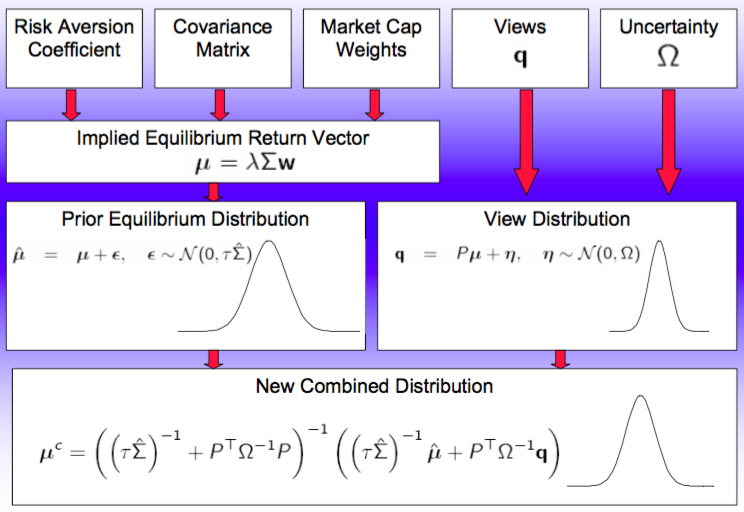
\includegraphics[width=1.0\linewidth]{BL_Roadmap}
%\caption{The roadmap to the BL approach}
%\label{Fig_BLRoadmap}
%\end{figure}

\subsection{The Math Behind Black-Litterman}

\paragraph{Main assumptions}
\begin{itemize}
\item \emph{Market structure:}
\begin{itemize}
\item $n$ assets
\item expected return vector $\bm \mu \in \mathbb{R}^{n \times 1}$
\item expected covariance matrix $\Sigma \in \mathbb{R}^{n \times n}$
\end{itemize}
\item \emph{Investors:}
\begin{itemize}
\item quadratic utility function / static optimization problem:
\begin{align*}
\max_{\bm w} \left( \bm w^\top \bm \mu + (1-\bm w^\top \bm 1) R_f - \frac{\lambda}{2} \bm w^\top \Sigma \bm w \right)
\end{align*}
where $\lambda$ is the risk aversion coefficient.
\end{itemize}
\end{itemize}

\subsubsection{Step 1: Equilibrium as Reference Point}

\paragraph{CAPM equilibrium return}
\begin{itemize}
\item CAPM equilibrium returns are the current market collective forecasts of next period returns ($\leadsto$ "prediction markets").
\item The market capitalization $\bm w$ (since we assume being in equilibrium) can be computed via:
\begin{itemize}
\item Approach with excess returns $\bm \mu - \bm 1 R_f$:
\begin{align*}
\bm w^\ast = \arg\max_{\bm w} \left( \bm w^\top \bm \mu + (1 - \bm w^\top \bm 1)R_f - \frac{\lambda}{2} \bm w^\top \Sigma \bm w \right)
\end{align*}
which leads to:
\begin{align*}
\bm \mu - \bm 1 R_f &= \lambda \Sigma \bm w^\ast \quad \Rightarrow \quad
\bm w^\ast = (\lambda \Sigma)^{-1} (\bm \mu - \bm 1 R_f)
\end{align*}
\item Approach with returns $\bm \mu$ (cf. application section):
\begin{align*}
\bm w^\ast = \arg\max_{\bm w} \left( \bm w^\top \bm \mu - \frac{\lambda}{2} \bm w^\top \Sigma \bm w \right), \qquad \lambda \approx 3
\end{align*}
which leads to:
\begin{align*}
\bm \mu = \lambda \Sigma \bm w^\ast \quad \Rightarrow \quad
\bm w^\ast = (\lambda \Sigma)^{-1} \bm \mu
\end{align*}
\end{itemize}
\item The risk aversion coefficient $\lambda$:
\begin{enumerate}
\item can be computed via the market's excess return $\mu_m$ and its variance $\sigma_m^2$:
\begin{align*}
\lambda &= \frac{\mu_m}{\sigma_m^2}
\end{align*}
\item or can be calibrated to the \textit{historical Sharpe ratio}, e.g. often $\lambda \approx 3$.
\end{enumerate}
\end{itemize}

\paragraph{Note on estimation errors}
\begin{itemize}
\item Estimation cannot directly be derived (since equilibrium returns are not actually estimated).
\item But the following is known: \\
The estimation error of the means of returns should be less than the covariance fo the returns.
\item Practical approach: \\
Define estimation error proportional to the covariance matrix of returns via a scalar $\tau$, e.g. $\tau \Sigma$ with $\tau < 1$.
\item Setting of $\tau$: (very different approaches)
\begin{itemize}
\item $\tau \in [0.01, 0.05]$ \\
since: The uncertainty in the mean is less than the uncertainty in the variance, thus $\tau$ should be close to zero.
\item $\tau = 1$ (missing justification \ldots)
\item often $\tau = 0.3$ (another arbitrary choice)
\item $\tau = 1 / \text{number of observations}$ \\
since: $\tau \Sigma$ is interpreted as the standard error of the estimate of the implied equilibrium return vector.
\end{itemize}
\end{itemize}

\paragraph{Prior distribution}
The prior distribution of expected returns is $\mathcal{N}(\bm \mu, \tau \hat \Sigma)$, where $\hat \Sigma$ is the estimated covariance matrix.

\subsubsection{Step 2: Our Views}

\paragraph{Characteristics of views}
\begin{itemize}
\item Each view is unique and uncorrelated with other views. \\
($\leadsto$ improved stability and simplification of the problem)
\item A view on every asset is NOT required --- views may even conflict.
\item two types of views:
\begin{itemize}
\item \textit{absolute view:} sum of weights is one
\item \textit{relative view:} sum of weights is zero \\
Note: relative view weights on a group of assets can either be equal ($\leadsto \frac{1}{n}$) or account for relative market capitalization.
\end{itemize}
\end{itemize}

\paragraph{Formulation of views}
\begin{itemize}
\item \textit{view vector:}
\begin{align*}
\bm q = P \bm \mu + \bm \eta, \qquad \eta \sim \mathcal{N}(0, \Omega), \qquad P \in \mathbb{R}^{k \times n}, \quad \Omega \in \mathbb{R}^{k \times k}
\end{align*}
i.e. there are $k$ views for a market with $n$ assets.
\item \textit{view portfolios $P \mu$:} each row represents a weight vector of $n$ assets, i.e. $P \mu$ expresses our views via $k$ view portfolios. \\
Note that $P$ is not required to be invertible.
\item \textit{confidence/covariance of view portfolios $\Omega$:} \\
there appear to be two approaches presented in the lecture:
\begin{itemize}
\item directly based on \textit{investors' confidences:}
\begin{align*}
\Omega &= \diag(\omega_1, \ldots, \omega_k)
\end{align*}
\item based on \textit{historical estimates:}
\begin{align*}
\Omega &= \tau \diag(\bm p_1 \hat \Sigma \bm p_1^\top, \ldots, \bm p_k \hat \Sigma \bm p_k^\top)
\end{align*}
with $P = (\bm p_1^\top, \ldots, \bm p_k^\top)^\top$ and $\hat \Sigma$ the historical estimate of the real covariance matrix $\Sigma$.
\end{itemize}
\end{itemize}

\subsubsection{Step 3: Combining Equilibrium and View}

\paragraph{Derivation}
\begin{itemize}
\item Given:
\begin{itemize}
\item expected returns:
\begin{align*}
\hat{\bm \mu} &= \bm \mu + \bm \epsilon, \qquad \bm \epsilon \sim \mathcal{N}(0, \tau \hat \Sigma)
\end{align*}
\item views:
\begin{align*}
\bm q &= P \bm \mu + \bm \eta, \qquad \bm \eta \sim \mathcal{N}(0, \Omega)
\end{align*}
\end{itemize}
\item Define the following:
\begin{align*}
\bm y &= (\hat{\bm \mu}, \bm q)^\top \in \mathbb{R}^{n+k} & X &= (I, P^\top)^\top \in \mathbb{R}^{(k+n) \times n} \\
\bm u &= (\bm \epsilon, \bm \eta)^\top \in \mathbb{R}^{n+k} & \psi &= \diag(\tau \hat \Sigma, \Omega) \in \mathbb{R}^{(n+k) \times (n+k)}
\end{align*}
with $\bm u \sim \mathcal{N}(0, \psi)$
\item \textit{Regression equation:}
\begin{align*}
\bm y &= X \bm \mu + \bm u
\end{align*}
\item \textit{Generalized least-square estimator:}
\begin{align*}
\bm \mu^c &= (X^\top \psi^{-1} X)^{-1} X^\top \psi^{-1} \bm y \quad \in \mathbb{R}^n
\end{align*}
\end{itemize}

\paragraph{BL Master Formula}
\begin{align*}
\bm \mu^c& = \underbrace{\left( (\tau \hat \Sigma)^{-1} + P^\top \Omega^{-1} P \right)^{-1}}_\text{normalization factor} \cdot \underbrace{\left( (\tau \hat \Sigma)^{-1} \hat{\bm \mu} + P^\top \Omega^{-1} \bm q \right)}_\text{weighting factors: eq. returns \& views} \\
&= \hat{\bm \mu} + \tau \hat \Sigma P^\top \left( \tau P \hat \Sigma P^\top + \Omega \right)^{-1} (\bm q - P \hat{\bm \mu})
\end{align*}

\paragraph{Variance of $\mu^c$}
\begin{align*}
(\sigma^c)^2 &= \left( (\tau \hat \Sigma)^{-1} + P^\top \Omega^{-1} P \right)^{-1}
\end{align*}
(which corresponds to the normalization factor in the BL master formula)

\paragraph{Limiting cases}
consider:
\begin{multicols*}{2}
\begin{itemize}
\item case $\bm \mu^c = \hat{\bm \mu}$:
\begin{itemize}
\item no view: $P=0$
\item no confidence: $\Omega \rightarrow \infty$
\item no estimation error: $\tau \rightarrow 0$
\end{itemize}
\item case $\bm \mu^c = P^{-1} \bm q$:
\begin{itemize}
\item absolute confidence: $\Omega \rightarrow 0$
\item infinite estimation error: $\tau \rightarrow \infty$
\end{itemize}
\end{itemize}
\end{multicols*}

\subsubsection{Step 4: Optimization}

Markowitz optimization with adjusted mean $\mu^c$ and given estimated covariance matrix $\hat \Sigma$, which gives the whole efficient frontier.
\begin{align*}
\bm w^c &= \frac{1}{\lambda} \hat \Sigma^{-1} \bm \mu^c \\
&= \bm w + P^\top \left( P \hat \Sigma P^\top + \frac{1}{\tau} \Omega \right)^{-1} \left( \frac{1}{\lambda} \bm q - P \hat \Sigma \bm w \right)
\end{align*}
Often, $\Omega$ is specified as $\Omega = \diag \left[ P \hat \Sigma P^\top \right] \tau$ to make $w^c$ independent of $\tau$.

\section{Bayesian Mean Variance Analysis and Shrinkage}

\paragraph{Overview}
\begin{itemize}
\item As the BL model, Bayesian analysis provides a method to incorporate an investor's prior information into the estimation of mean returns.
\item In principle, incorporating prior information about the covariance matrix of returns is also possible.
\item Including prior information reduces over-fitting and smoothes out the influence of the particular sample available.
\end{itemize}

\subsection{Basic Bayes}

\paragraph{Likelihood function}
\begin{itemize}
\item given: data series $Y$ and model with unknown parameter $\theta$
\item joint density function of $Y$ for a given value of $\theta$: $f(y_1, \ldots, y_m | \theta)$
\item vs. likelihood function: $L(\theta | y_1, \ldots, y_m) = f(y_1, \ldots, y_m | \theta)$
\end{itemize}

\paragraph{Bayes theorem}
\begin{itemize}
\item Bayes rule:
\begin{align*}
\mathbb{P}[E | D] &= \frac{\mathbb{P}[E \cap D]}{\mathbb{P}[D]} = \frac{\mathbb{P}[D | E]}{\mathbb{P}[D]} \cdot \mathbb{P}[E]
\end{align*}
i.e.
\begin{align*}
\mathbb{P}[E | D] \cdot \mathbb{P}[D] &= \mathbb{P}[D | E] \cdot \mathbb{P}[E]
\end{align*}
\item Bayes theorem consists of the following elements:
\begin{itemize}
\item $\mathbb{P}[D | E]$: \textit{likelihood} \\
i.e. the conditional probability of the new data given that the prior evidende $E$ is true
\item $\mathbb{P}[D]$: \textit{evidence} \\
i.e. the unconditional probability of the additional data (new observation)
\item $\mathbb{P}[E]$: \textit{prior} probability \\
i.e. the prior belief \\
i.e. the probability of the evidence before the additional data (new observation)
\item $\mathbb{P}[E | D]$: \textit{posterior} probability \\
i.e. probability of the evidence after the additional data (new observation)
\end{itemize}
which can be summarized as:
\begin{align*}
\text{posterior} &= \frac{\text{likelihood}}{\text{evidence}} \text{prior}
\end{align*}
\item \textit{Remarks:}
\begin{itemize}
\item Updated posterior beliefs are the result of a tradeoff between prior and data distributions.
\item The degree of the tradeoff is determined by the strength of the prior and the amount of available data.
\end{itemize}
\end{itemize}

\paragraph{Priors}
\begin{itemize}
\item \textit{Informative} prior elicitation
\begin{itemize}
\item modify sustantially the information contained in the sample
\item also enclose information about the spread of the distribution
\end{itemize}
\item \textit{Noninformative} prior distribution
\begin{itemize}
\item vague or diffuse priors are often modeled via uniform distribution or Jeffrey's prior
\item may be improper (i.e. do not integrate to one) --- although resulting densities are usually proper
\end{itemize}
\item \textit{Conjugate} prior distribution
\begin{itemize}
\item choice of prior often governed by aim to obtain analytically tractable solution
\item $\leadsto$ conjugate prior distributions guarantee that the posterior distribution is of the same class as the prior distribution
\end{itemize}
\end{itemize}

\subsection{A Simple Bayesian Model}

\begin{itemize}
\item case: unknown mean $\mu \sim \mathcal{N}(\hat \mu, \hat \sigma_\mu^2)$, known variance $\sigma_0^2$
\item aim: find mean $\hat \mu$ and variance $\hat \sigma_\mu^2$ of the unknown mean $\mu$
\item data distribution:
\begin{align*}
X | \mu, \sigma_0^2 &\sim \mathcal{N}(\mu, \sigma_0^2) = \frac{1}{\sqrt{2\pi \sigma_0^2}} \exp \left( -\frac{1}{2\sigma_0^2} (X-\mu)^2 \right)
\end{align*}
\item normal prior distribution (for unknown mean):
\begin{align*}
\mu | r,s^2 &\sim \mathcal{N}(r,s^2)
\end{align*}
with $r,s$ known
\item after computing the posterior distribution $\mathbb{P}[\mu | \bm x] \propto \mathbb{P}[\bm x | \mu] \mathbb{P}[\mu]$, the following \textit{point estimates} are obtained:
\begin{align*}
\hat \mu &= \frac{\frac{r}{s^2} + \frac{m \bar x}{\sigma_0^2}}{\frac{1}{s^2} + \frac{m}{\sigma_0^2}}, \qquad
\hat \sigma_\mu^2 = \left( \frac{1}{s^2} + \frac{m}{\sigma_0^2} \right)^{-1}
\end{align*}
where $r,s,\sigma_0^2$ are known, $\bar x$ is the mean of the data set and $m$ denotes the number of data points.
\item Characteristics:
\begin{itemize}
\item prior precision: $1/s^2$
\item data precision: $m/\sigma_0^2$
\item posterior precision: $1/s^2 + m/\sigma_0^2$
\end{itemize}
\item Note that for an infinite amount of data, i.e. $m \to \infty$:
\begin{align*}
\lim_{m \to \infty} \hat \mu = \bar x, \qquad \lim_{m \to \infty} \hat \sigma_\mu^2 = 0
\end{align*}
\item \textit{Remarks:}
\begin{itemize}
\item non-Gaussian prior could have been adopted as well
\item uniform prior: possible, but does not change the posterior from the sample mean
\item prior could also be placed on variance, but this is not important in practice
\end{itemize}
\end{itemize}

\subsection{Bayesian Portfolio Selection}

\paragraph{Excess returns}
\begin{itemize}
\item Predictive return density of the yet unobserved next-period excess return $R_{T+1}$:
\begin{align*}
p(R_{T+1} | R) &= \int p(R_{T+1}| \bm \mu, \Sigma) p(\bm \mu, \Sigma | R) d\bm  \mu d\Sigma
\end{align*}
where $R \in \mathbb{R}^{T \times n}$, $p(\bm \mu, \Sigma | R)$ the joint posterior density of the two parameters of the multivariate normal and $p(R_{T+1} | \bm \mu, \Sigma)$ is the multivariate normal density.
\item \textit{Remark:} averaging over the posterior distribution accounts for estimation risk.
\item In the multivariate normal setup:
\begin{align*}
L(\bm \mu, \Sigma | R) \propto |\Sigma|^{-T/2} \exp \left( -\frac{1}{2} \sum_{t=1}^T (R_t - \bm \mu)^\top \Sigma^{-1} (R_t - \bm \mu) \right)
\end{align*}
\end{itemize}

\paragraph{Scenario 1: MV with diffuse (improper) priors}
\begin{itemize}
\item Assume: investor has \textit{no particular prior knowledge} of the distribution parameters $\bm \mu$ and $\Sigma$.
\item typical choice: \emph{Jeffreys' prior}
\begin{align*}
p(\bm \mu, \Sigma) \propto |\Sigma|^{-(n+1)/2}
\end{align*}
\item Predicitive distribution of the excess return is a multivariate Student's t-distribution with $T-n$ degrees of freedom.
\item Then: predictive mean and covariance matrix of returns:
\begin{align*}
\bm{\tilde \mu} = \bm{\hat \mu}, \qquad \tilde \Sigma = \frac{(1+1/T)(T-1))}{T-n-2} \hat \Sigma
\end{align*}
with the sample estimate:
\begin{align*}
\hat \Sigma = \frac{1}{T-1} \sum_{t=1}^T (R_t - \bm{\hat \mu}) (R_t - \bm{\hat \mu})^\top
\end{align*}
\item \emph{Interpretation:} \\
Since the predictive expected return is not shrunk towards the prior mean, the full amount of any sampling error is transferred to the posterior mean. \\
Thus, scenario 1 is more appropriate when we do NOT suspect that the sample mean contains substaintial estimation errors.
\end{itemize}

\paragraph{Scenario 2: MV with proper priors}
\begin{itemize}
\item Assume: investor has \textit{informative beliefs} about the mean vector and the covariance matrix of return. \\
Here: \textit{conjugate priors:}
\begin{itemize}
\item conjugate prior of the mean vector of the normal distribution: multivariate normal:
\begin{align*}
\bm \mu | \Sigma \sim \mathcal{N} \left( \bm \eta, \frac{1}{\tau} \Sigma \right)
\end{align*}
where $\tau$ determines the strength of the confidence in $\bm \eta$. \\
(e.g. if $\tau = 0$, then the investor has no knowledge and the variance of $\mu$ becomes infinite, thus the means becomes uniformly distributed on $\mathbb{R}$)
\item conjugate prior of the unknown covariance matrix of the normal distribution: inverted Whishart distribution:
\begin{align*}
\Sigma \sim \IW(\Omega, \nu)
\end{align*}
where $\nu$ refelcts the confidence in $\Omega$.
\end{itemize}
\item Then: predicitve distribution of next-period's excess returns are multivariate Student's t with:
\begin{align*}
\bm{\tilde \mu} &= \frac{\tau}{T+\tau} \eta + \frac{T}{T+\tau} \bm{\hat \mu} \\
\tilde \Sigma &= \frac{T+1}{T(\nu+n-1)} \left( \Omega + (T-1)\hat \Sigma + \frac{T \tau}{T+\tau} (\bm \eta - \bm{\hat \mu}) (\bm \eta - \bm{\hat \mu})^\top \right)
\end{align*}
\item \textit{Remark:} In contrast to scenario 1, the predictive mean and covariance matrix are not proportional to the sample estimates $\bm{\hat \mu}$ and $\hat \Sigma$.
\item \emph{Interpretation:} \\
The predictive mean is a weighted average for the prior mean $\bm \eta$ and the sample mean $\bm{\hat \mu}$. \\
Thus, the sample mean is shrunk towards the prior mean. The stronger the belief in the prior mean, the larger the degreee to which the prior mean influences the predictive mean.
\end{itemize}

\subsection{Shrinking $\mu$}

\paragraph{Admissible estimator}
Let $X$ be a RV with distribution depending on an unknown parameter $\mu$ lying in a parameter space $\Theta$. Let $\delta$ denote an estimator of $\mu$.
\begin{itemize}
\item An estimator $\delta_1$ is \textit{as good as} an estimator $\delta_2$ if:
\begin{align}
R(\mu,\delta_1) \leq R(\mu,\delta_2), \forall \mu \in \Theta
\label{Eq_EstAsGoodAs}
\end{align}
\item An estimator $\delta_1$ is \textit{better than} an estimator $\delta_2$ if eq. (\ref{Eq_EstAsGoodAs}) is satisfied and:
\begin{align*}
R(\mu,\delta_1) < R(\mu,\delta_2) \quad \text{for at least one } \mu \in \Theta.
\end{align*}
\item An estimator is said to be \textit{admissible} if there exists no estimator which is better than that. \\
Otherwise, it is an \textit{inadmissible} estimator.
\end{itemize}

\paragraph{Stein-James shrinkage estimator}
\begin{itemize}
\item Consider $X_t \sim \mathcal{N}(\bm \mu, \Sigma)$ with $X_t \in \mathbb{R}^n$, $n > 2$, $t = 1, \ldots, T$.
\item Stein-James shrinkage estimator:
\begin{align*}
\hat \delta_a = (1-w) \bm{\hat \mu} + w \bm b, \qquad w = \frac{a}{(\bm{\hat \mu} - \bm b)^\top (\bm{\hat \mu} - \bm b)}
\end{align*}
with $\bm{\hat \mu} = \frac{1}{T} \sum_t X_t \sim \mathcal{N}(\bm \mu, \Sigma/T)$ the sample mean, $\bm b$ any constant vector and $a$ any scalar s.t.
\begin{align*}
0 < a < \frac{2}{T} (\tr(\Sigma) - 2 \lambda_1)
\end{align*}
where $\lambda_1$ is the largest eigenvalue fo the matrix $\Sigma$, for which it must hold $(\tr(\Sigma) - 2 \lambda_1) > 0$.
\item The MSE using $\bm{\hat \delta}_a$ is smaller than the MSE from using $\bm{\hat \mu}$.
\end{itemize}

\section{Regime Swiching and Asset Allocation}

\paragraph{Motivation}
\begin{itemize}
\item A RS model allos the data to be drawn from two or more possible distributions (regimes).
\item e.g. two regimes for international equity returns: \\
a \textit{normal regime} and a \textit{bear regime} with:
\begin{itemize}
\item lower average returns
\item higher volatility
\item higher correlation
\end{itemize}
\end{itemize}

\subsection{A Simple RS Model}

\paragraph{Serially uncorrelated data}
\begin{itemize}
\item Regression model \textit{without} switching:
\begin{align*}
y_t &= \beta x_t + e_t, \qquad e_t \sim \text{i.i.d.} \mathcal{N}(0, \sigma^2)
\end{align*}
To estimate this model, simply maximize the log-likelihood function w.r.t. $beta$ and $\sigma^2$:
\begin{align*}
\log L = \sum_{t=1}^T \log f(y_t), \qquad
f(y_t) = \frac{1}{\sqrt{2 \pi \sigma^2}} \exp \left( -\frac{(y_t - \beta x_t)^2}{2 \sigma^2} \right)
\end{align*}
\item Now: regression with \textit{structural breaks:}
\begin{align*}
y_t &= \beta_{S_t} x_t + e_t, \qquad e_t \sim \text{i.i.d.} \mathcal{N}(0, \sigma_{St}^2)
\end{align*}
with:
\begin{align*}
\beta_{S_t} &= \beta_0 (1-S_t) + \beta_1 S_t, \qquad \sigma_{S_t}^2 = \sigma_0^2 (1-S_t) + \sigma_1^2 S_t
\end{align*}
and $S_t \in \lbrace 0,1 \rbrace$. \\
If $S_t$ is known for $t = 1,2,\ldots,T$, the same log-likelihood function as before can be maximized w.r.t. $\beta_0, \beta_1, \sigma_0, \sigma_1$.
\end{itemize}

\paragraph{Markov switching}
\begin{itemize}
\item If $S_t$ is not known a priori, then the following two-step procedure has to be applied:
\item \textit{Step 1:} decompose the joint density of $y_t$ and unobserved $S_t$:
\begin{align*}
f(y_t,S_t | \mathcal{F}_{t-1}) &= f(y_t | S_t, \mathcal{F}_{t-1}) f(S_t | \mathcal{F}_{t-1})
\end{align*}
After integrating $S_t$ our of the joint density $f(y_t | \mathcal{F}_{t-1})$, the log-likelihood function is then given by:
\begin{align*}
\log L &= \sum_{t=1}^T \log f(y_t | \mathcal{F}_{t-1}) \\
&= \sum_{t=1}^T \log \left( \sum_{S_t=0}^1 f(y_t | S_t, \mathcal{F}_{t-1}) \mathbb{P}[S_t | \mathcal{F}_{t-1}] \right)
\end{align*}
which is a weighted average of the conditional densities given $S_t = 0$ and $S_t = 1$. \\
To calculate $\mathbb{P}[S_t | \mathcal{F}_{t-1}]$, a priori assumptions need be made about the behaviour of $S_t$.
\item \emph{Independent Switching}
\begin{itemize}
\item Assume: $S_t$ evolves independently of its own past values.
\item possible specification:
\begin{align*}
\mathbb{P}[S_t = 1] &= p = \frac{\exp(p_0)}{1 + \exp(p_0)}, \qquad \mathbb{P}[S_t = 0] = 1-p
\end{align*}
where $p_0$ is an unconstrained parameter.
\item If $S_t$ does not depend on any other exogenous parameter, then the log-likelihood function can simply be maximized w.r.t. $\beta_0, \beta_1, \sigma_0, \sigma_1$ and $p_0$.
\item If $S_t$ evolves independently of its own past values, but depends on some exogenous variable $Z_{t-1}$, then e.g.
\begin{align*}
\mathbb{P}[S_t = 1 | \mathcal{F}_{t-1}] &= p_t = \frac{\exp(p_0 + Z_{t-1} p_1)}{1 + \exp(p_0 + Z_{t-1} p_1)} \\
\mathbb{P}[S_t = 0 | \mathcal{F}_{t-1}] &= 1-p_t
\end{align*}
and the log-likelihood function can be maximized additionally w.r.t. $p_1$.
\end{itemize}
\item \emph{Markov Switching}
\begin{itemize}
\item Assume: $S_t$ depends on past values of $S_t$. \\
Consider here: the simplest case of an $r^{th}$ order Markov, i.e. a first-order Markov switching process for $S_t$.
\item Then: transition probabilities:
\begin{align*}
\mathbb{P}[S_t &= 1 | S_{t-1} = 1] = p = \frac{\exp(p_0)}{1 + \exp(p_0)} \\
\mathbb{P}[S_t &= 0 | S_{t-1} = 0] = q = \frac{\exp(q_0)}{1 + \exp(q_0)}
\end{align*}
\item Apply the following \emph{filter:}
\begin{enumerate}
\item Given $\mathbb{P}[S_{t-1} = i | \mathcal{F}_{t-1}]$, $i = 0,1$ at the beginning of time $t$, the weighting terms are calculated as:
\begin{align*}
\mathbb{P}[S_t = j | \mathcal{F}_{t-1}] = \sum_{i=0}^1 \mathbb{P}[S_t = j | S_{t-1} = i] \mathbb{P}[S_{t-1} = i | \mathcal{F}_{t-1}]
\end{align*}
\item Once $y_t$ is observed at the end of time $t$, update the probability term:
\begin{align*}
\mathbb{P}[S_t = j | \mathcal{F}_t] = \frac{f(y_t | S_t = j, \mathcal{F}_{t-1}) \mathbb{P}(S_t = j | \mathcal{F}_{t-1})}{\sum_{k=0}^1 f(y_t | S_t = k, \mathcal{F}_{t-1}) \mathbb{P}(S_t = k | \mathcal{F}_{t-1})}
\end{align*}
\end{enumerate}
\item Repeat the above steps to get $\mathbb{P}[S_t = j | \mathcal{F}_{t-1}]$, $t=1,\ldots,T$.
\item To start the filter, $\mathbb{P}[S_0^ | \mathcal{F}_0]$ is required. Thus, emply the steady-state or unconditional probabilities of $S_t$:
\begin{align*}
\pi_0 = \frac{1-p}{2-p-q}, \qquad \pi_1 = \frac{1-q}{2-p-q}
\end{align*}
\item Finally, optimize the log-likelihood function:
\begin{align*}
\log L &= \sum_{t=1}^T \log \left( \sum_{S_t=0}^1 f(y_t | S_t, \mathcal{F}_{t-1}) \mathbb{P}[S_t | \mathcal{F}_{t-1}] \right)
\end{align*}
w.r.t. $\beta_0, \beta_1, \sigma_0, \sigma_1, p$ and $q$.
\end{itemize}
\end{itemize}

\paragraph{Steady-state probabilities}
\begin{itemize}
\item Transition probabilities of a first-order, $M$-state Markov switching process:
\begin{align*}
P = \begin{bmatrix}
p_{11} & p_{12} & \ldots & p_{1M} \\
p_{21} & p_{22} & \ldots & p_{2M} \\
\vdots & \vdots & \ddots & \vdots \\
p_{M1} & p_{M2} & \ldots & p_{MM}
\end{bmatrix}, \qquad
P \bm 1 = \bm 1
\end{align*}
\item Then the steady-state probabilitie can be obtained by:
\begin{align*}
\bm \pi_t = (A^\top A)^{-1} A^\top \begin{bmatrix} 0_M \\ 1 \end{bmatrix}
\end{align*}
i.e. the steady-state probabilities are the last column of the matrix $(A^\top A)^{-1} A^\top$.
\end{itemize}

\subsection{Application: International CAPM}

\paragraph{The Model}
\begin{itemize}
\item International CAPM model with world market return:
\begin{align*}
y_t^w &= \mu^w + \sigma^w \epsilon_t^w, \qquad \epsilon_t^w \sim \mathcal{N}(0,1)
\end{align*}
\item Now: introduce two states, $s=1,2$, with conditional world mean world volatility $\mu_s^w$ and $\sigma_s^w$ (no country-specific regimes).
\end{itemize}

\paragraph{Regime dynamics}
\begin{itemize}
\item For each point in time, the portfolio managers knows the realized regime, but does not know which regime will be realized in the next time period.
\item The regime follows a Markov process with constant transition probabilities $q$ and $p$. \\
Note that usually $p = 1-q$ is not realistic. Empirical studies found that both $p$ and $q$ are well above 0.5, indicating \textit{persistent states}.
\end{itemize}

\paragraph{Expected excess returns}
\begin{itemize}
\item Expected excess return of country $j$ is given by:
\begin{align*}
e_{j,i} &= (1-\beta^j) \mu^z + \beta^j e_i^w
\end{align*}
where $i$ is the prevailing regime and $e_i^w$ is the world's expected excess return, $i=1,2$.
\item Expected excess returns differ across individual equity indices only through their different betas w.r.t. the world market.
\end{itemize}

\paragraph{Covariance matrix}
\begin{itemize}
\item Add \textit{idiosyncratic} part $V = \diag(\bar \sigma_j^2) \in \mathbb{R}^{J \times J}$
\item Add a \textit{regime-dependent systematic} part.
\item Then:
\begin{align*}
\Omega_i &= (\bm \beta \bm \beta^\top) (\sigma^w(S_{t+1} = i))^2 + V, \qquad i = 1,2
\end{align*}
\item Take current regimes into account. \\
Depending on which regime we are at the current time, we get different covariance matrices:
\begin{align*}
\Sigma_1 &= p \Omega_1 + (1-p) \Omega_2 + p(1-p)(\bm e_1 - \bm e_2) (\bm e_1 - \bm e_2)^\top \\
\Sigma_2 &= q \Omega_2 + (1-q) \Omega_1 + q(1-q)(\bm e_1 - \bm e_2) (\bm e_1 - \bm e_2)^\top
\end{align*}
\end{itemize}

%\subsection{Application: Market Timing}
% -> not relevant for exam

\columnbreak
\begin{center}
\textit{intentionally left blank}
\end{center}
\vfill

\section*{Notations}

Unless otherwise specified, the following notations were used:
\begin{description}[style=multiline,leftmargin=1cm,font=\textbf]
\item[$\phi$] standard normal PDF
\item[$\Phi$] standard normal CDF
\end{description}

\section*{Abbreviations}

\begin{description}[style=multiline,leftmargin=1cm,font=\textbf]
%\item[a.a.] almost all
%\item[a.s.] almost surely
%\item[BM] Brownian motion
\item[CDF] cumulative distribution function
\item[cf.] conferre
\item[e.g.] exempli gratia
\item[i.e.] id est
\item[iff] if and only if
\item[IOT] in order to
%\item[PDE] partial differential equation
\item[PDF] probability density function
%\item[RCLL] right-continuous with left limits
\item[RV] random variable
%\item[SDE] stochastic differential equation
\item[s.t.] such that
\item[w.r.t.] with respect to
\end{description}

\section*{Disclaimer}

\begin{itemize}
\item This summary is work in progress, i.e. neither completeness nor correctness of the content are guaranteed by the author.
\item This summary may be extended or modified at the discretion of the readers.
\item Source: Lecture \SummaryTitle, \SummarySemester, UZH (lecture notes, script, exercises and literature). Copyright of the content is with the lecturers.
\item The layout of this summary is based on the summaries of several courses of the BSc ETH ME from Jonas LIECHTI.
\end{itemize}

\end{multicols*}

\end{document}